\documentclass[letter,12pt]{article}
\usepackage[letterpaper,right=1in,left=1in,top=1in,bottom=1in]{geometry}
\usepackage{setspace}
\onehalfspacing

\usepackage[utf8]{inputenc}   % allows input of special characters from keyboard (input encoding)
\usepackage[T1]{fontenc}      % what fonts to use when printing characters       (output encoding)
\usepackage{amsmath}          % facilitates writing math formulas and improves the typographical quality of their output
\usepackage[hyphens]{url}     % adds line breaks to long urls
\renewcommand{\UrlFont}{\ttfamily\small} % shrinks url font 1 step down
\urlstyle{tt}                 % how urls appear, options tt rm sf and same, see https://mirrors.mit.edu/CTAN/macros/latex/contrib/url/url.pdf
\usepackage[pdftex]{graphicx} % enhanced support for graphics
\usepackage{tikz}             % Easier syntax to draw pgf files (invokes pgf automatically)
\usetikzlibrary{arrows}

\usepackage{mathptmx}           % set font type to Times
\usepackage[scaled=.90]{helvet} % set font type to Times (Helvetica for some special characters)
\usepackage{courier}            % set font type to Times (Courier for other special characters)

% \usepackage[longnamesfirst, sort]{natbib}\bibpunct[]{(}{)}{,}{a}{}{;} % handles biblio and references 
\usepackage[sort]{natbib}\bibpunct[]{(}{)}{,}{a}{}{;} % handles biblio and references 

\usepackage{rotating}         % sideway tables and figures that take a full page
\usepackage{caption}          % allows multipage figures and tables with same caption (\ContinuedFloat)

\usepackage{dcolumn}          % needed for apsrtable and stargazer tables from R to compile
\usepackage{arydshln}         % dashed lines in tables (hdashline, cdashline{3-4}, 
                              %see http://tex.stackexchange.com/questions/20140/can-a-table-include-a-horizontal-dashed-line)
                              % must be loaded AFTER dcolumn, 
                              %see http://tex.stackexchange.com/questions/12672/which-tabular-packages-do-which-tasks-and-which-packages-conflict


\newcommand{\mc}{\multicolumn}

%% TO ADD NOTES IN TEXT, PUT % BEFORE THE ONE YOU WANT DISABLED
%\usepackage[disable]{todonotes}                            % no show
\usepackage[colorinlistoftodos, textsize=small]{todonotes} % show notes
\newcommand{\emm}[1]{\todo[color=red!15, inline]{\textbf{Eric:} #1}}

%% \usepackage{xr} % allows cross-ref to other file
%% \externaldocument{urge15appendix}

%% %for submission: sends figs, tables, and footnotes to last pages
%% \RequirePackage[nomarkers,nolists]{endfloat}     % sends tables and figures to the end
%% \RequirePackage{endnotes}                        % turns fn into endnotes; place \listofendnotes where you want 
%%                                                  %the endnotes to appear (it must be after the last endnote).
%% \let\footnote=\endnote
%% \newcommand{\listofendnotes}{
%%    \begingroup
%%    \parindent 0pt
%%    \parskip 2ex
%%    \def\enotesize{\normalsize}
%%    \theendnotes
%%    \endgroup
%% }

%% % for submission: drop page numbers when producing title page
%% \pagenumbering{gobble} % Remove page numbers (and reset to 1)
%% \pagenumbering{arabic}% Arabic page numbers (and reset to 1)

\setcitestyle{citesep={;}}

\usepackage{hyperref}

\usepackage{bigfoot}  %% allows the use of \verb command within footnotes

\usepackage{epigraph}
\setlength\epigraphrule{0pt} % no rule under the epigraph

\begin{document}

\title{Local Competition in Mexican Politics since 1979: \\ A Comprehensive Dataset of Municipal Elections}
\author{Eric Magar\footnote{The author is grateful for financial support for research from the Asociación Mexicana de Cultura \textsc{a.c.} and for research assistance by Gabino Martínez Díaz, Isaac Palatto Sánchez, Rodrigo Santibáñez Razo, and Carlos Alexis Sarabia Melgarejo. All remaining errors are my own.} \\ ITAM \\ \url{emagar@itam.mx}}
\date{\today}
%\date{December 11, 2025 \\ Under review by \emph{Mexican Studies/Estudios Mexicanos}}
\date{May 20, 2026 \\ Under review by \emph{Mexican Studies/Estudios Mexicanos}}
%\date{May 20, 2026 \\ Conditionally accepted by \emph{Mexican Studies/Estudios Mexicanos}}
% \date{\today \\ Preliminary draft, please inquire for a newer version}
\maketitle

\begin{abstract}
\noindent I introduce a publicly available dataset of vote returns for Mexican municipal elections between 1979 and 2025. The dataset includes more than 35,000 races and provides municipality-level aggregates for votes won by each party, the number of registered voters, the number of candidates competing, the winner's name, the election date and its concurrence with other races, and identification codes for merging socio-demographic data. I present the data sources, explain the standardization of the time-series cross-sectional structure, and provide descriptive statistics. Patterns in the data are consistent with existing knowledge of Mexican elections and demostrate several promising applications of the dataset.
\end{abstract}

%% \begin{footnotesize}
%% \noindent \textbf{Keywords:} Municipal elections, elected municipal executive officers, consecutive reelection, electoral concurrence, systematized publicly-available datasets, democratization, 1979--2025, Mexico.
%% \end{footnotesize}

%% \bigskip

\epigraph{To Juan Molinar Horcasitas (1955--2015) pioneer of Mexican electoral studies \newline \emph{in memoriam}}

\newpage

\noindent The advent of partisan competition in Mexican politics coincided with the release of a wealth of public data across multiple areas of government. This development fueled a boom in the study of politics, public policy, and administrative processes in fields as diverse as the available data itself, including poverty alleviation, decentralized spending, public health, education, infrastruture, special interest groups, organized crime, and indigenous protest movements.\footnote{See \citet{diaz-estevez-magaloni-Poverty-book.2016, delao.cctransfers.2013, cantuGroceries2019, hernandez.jaramillo.FiscalDescentralMx2008wd, king.etal.segPop.2007, frenk.2006, behrman.etal.Prospera2025qe, avitabile.dehoyos.2018, garfias.etal.Infrastructure2021, palmer.rubin.Patronage2019cps, dube.garcia.ponce-MaizeDrugs2016jeea, dell.DrugWar.2015aer, timmons.broid.2013, trejo.Relig.indig.2009}.} These policy analyses are typically conducted using small units of observation, such as firms, schools, census tracts, or even individuals, yet the processes under study invariably intersect with municipal governments, and multivariate models commonly include controls at this level. Municipal election vote returns constitute a key input for empirical analysis.

This research note introduces a dataset of vote returns for Mexican municipal government elections over recent decades. Although vote returns are public information and can generally be found online with relative ease, the primary sources are dispersed across state-level websites, lack standardized reporting formats, contain many missing or incomplete years, and in some cases have been---or are at risk of being---removed because of insufficient funding. These limitations underscore the importance of maintaining a secondary source. The present dataset is distributed through a publicly available repository that consolidates municipal election results nationwide into a single comprehensive source. The data cover all municipalities that held local government elections between 1979 and 2025.

% \footnote{Early election scholars paid attention to federal elections for which vote returns have been rather well-organized and systematically available in public sources \citep[e.g.][]{gomezTagle.Estadisticas1990, segovia.dientes-sierra1983, molinar.1991a, segovia.els1979}. Discussion of state and municipal races was anecdotal at best due to data unavailability. The respository where the present dataset is distributed includes federal election vote returns too. This note centers in municipal elections only.} 

Repositories and websites that distribute historical vote returns for national legislative and executive elections at different levels of aggregation, free of charge, are numerous in both consolidated and consolidating democracies, including Mexico \citep{ife.2026}.\footnote{For instance, see \citet{mit.election.data.2017} and \citet{icpsr.us.hist.el.ret.2025} for U.S. presidential and Congressional elections since 1824; \citet{commons.library.uk.els.2023} for United Kingdom general elections since 1983; \citet{interieur.2026} and \citet{gougou.2025} for French presidential and National Assembly elections since 1958. Two remarkable endeavors systematizing and distributing a cross-national time-series of district-level election returns for the national assembly are \citet{lea.2009} and \citet{clea.2024}.} By contrast, efforts to compile and distribute historical vote returns for \emph{subnational} offices remain uncommon. This dataset joins a small number of similar initiatives in other countries of which I am aware, including a comprehensive database of U.S. local elections for 1989--2021 developed by \citet{am-loc-gov-els-database.2023}, the archive for local election results in Great Britain compiled by \citet{teale-loc-els-uk.2026}, and the dataset on the partisan composition of Swiss cantonal governments from 1848 to 2017 assembled by \citet{walter-emmenegger-Party-cantons-2018}. 

The note proceeds as follows. Section 1 describes municipal government authority and the relevant electoral institutions. Section 2 examines municipal party systems and introduces the principal contenders in these elections. Section 3 briefly discusses electoral fraud in Mexico. Section 4 details the data coverage and the organization of the distributed files. Section 5 provides an overview of pre-electoral coalitions in the units of observation, which pose an obstacle for some lines of research. Section 6 presents descriptive analyses of key variables in the dataset, comparing municipal patterns with findings from previous scholarship on federal, state, and subnational elections. Sections 7 and 8 describe additional datasets distributed alongside the main database, containing systematic information on elected municipal executives and electoral calendars, respectively, since 1989. Section 9 concludes.

\section{Municipal governments}

As of May 2025, Mexico's thirty-one states were subdivided into 2,460 municipalities, in addition to 17 municipality-equivalent jurisdictions in Mexico City, the nation's capital. \emph{Municipios} elect the lowest tier of government in Mexico's federal system. Because knowledge of subnational government and policy remains limited, I provide a brief institutional overview.

\subsection{Policy making and fiscal authority}

Municipal governments have constitutional authority over community policing, zoning and construction permits, drinking water provision, sewerage and waste disposal, street lighting, road paving, and park management, and they regulate public markets, slaughterhouses, and cemeteries. However, municipalities possess limited constitutional fiscal authority, raising only property taxes and user fees for public services. Historically, few municipalities invested in the administrative capacity necessary for effective revenue collection \citep{garfias.state.cap.2018}. Most municipalities---especially those in rural areas---derive the vast majority of their financial resources from federal revenue-sharing arrangements and earmarked federal transfers for public investment \citep{diaz.cayeros.2006, figueroa-mansur-itam.2024}.

Despite the limited scope of municipal authority, elected local officials appoint administrative staff and subcontract services and personnel, making municipal governments important sources of patronage within any spoils system. Local political organizations, and the resources they mobilize in pursuit of municipal office, are therefore central to the maintenance of state- and national-level parties \citep{ames.1970, coppedge.MxVen.1993, key.1964, rosas.lucardi.Brokers.2019}. For this reason, municipal politics occupies an important place in the study of politics and public policy.

With some exceptions, state capacity in Mexico is notoriously limited, particularly at the municipal level. In 2023, the median municipal government employed or contracted 13 bureaucrats per 1,000 registered voters, while the lower quartile employed 9 or fewer. By contrast, municipalities in the top decile employed 32 or more bureaucrats per 1,000 registered voters---roughly two and a half times the median level.\footnote{Descriptive statistics computed with data from the 2023 Municipal Government Census \citep{inegi.CensoGobMun2023}, excluding Mexico City and unelected municipalities.}

\subsection{Government structure}\label{S:structure}
Municipal authority is vested to a popularly elected body kown as the \emph{Ayuntamiento} (literally `yoked together'). The Ayuntamiento consists of the municipal council, or \emph{cabildo}, and a mayor---called \emph{presidente municipal} in some states, \emph{primer regidor} in others---and decisions are made by majority rule. The mayor serves as the chief executive officer, presides over council sessions with voice and a tie-breaking vote, and exercises varying appointment powers depending on the state \citep{robles-mtz.Municipio.2009, rmz-millan.2000}. The size of the cabildo is proportional to population. Councilors, known as \emph{regidores} or \emph{concejales}, hold ranked positions of precedence propose and propose and vote municipal policy through ordinances and regulations. In some states, the council also includes one or more \emph{síndicos}, officials responsible for treasury oversight and the municipality's legal representation. Síndicos may be either elected or appointed; appointed síndicos may speak in council sessions but do not have voting rights. Municipal governments possess no judicial authority, which instead resides with the states.

Although Mexico City is included in the dataset, I exclude it from the discussion below because of its special institutional status. Prior to 1997, the mayor of the Federal District was appointed by the president, and in turn appointed delegates to govern the city’s sixteen administrative jurisdictions, known as \emph{delegaciones}. Reforms enacted in 1997 converted all these positions into elected offices. The Federal District did not, however, acquire the status of a state, nor did the executives of the delegaciones obtain independent fiscal authority,  as taxation remained under the control of the city executive. Further reforms in 2018 introduced councils for the city's quasi-municipal jurisdictions---renamed \emph{alcaldías}---and formally changed the name of the Federal District to Mexico City \citep{rabell.2017}. 

\subsection{Electoral institutions}
Mayors are elected by plurality rule. In every municipality, regidores are elected through a mixed system in which one groups is chosen by plurality and another through proportional representation (PR). The ratio of plurality to PR regidores varies considerably across states. As of 2010, the average Ayuntamiento had a ratio of approximately $2:1$. In the state of Guanajuato, which had the lowest plurality share, the ratio was $1:4$, whereas in Tabasco, which had the highest plurality share, the ratio was the inverse , $4:1$ \citep[][:14]{gil.2010}. This institutional variation matters because higher numbers of PR regidores could leave the president in the council minority.

When plurality and PR seats are evenly balanced, however, the mayor necessarily enjoys majority status in the council because municipal officers are elected in fused tickets. Voters cast a single vote for a party list that includes the municipal president at the top of the ticket, followed by ranked regidores and, where applicable, síndicos. The vote is `fused' in the sense that it simultaneously determines the allocation of multiple offices \citep[see ][:42]{cox.1997}: the municipal presidency, all plurality regidor seats, and elected síndico psitions are awarded to the list receiving the most votes. The remaining regidor seats are then distributed proportionally across closed party lists. As a result, split-ticket voting is not technically possible.

\subsection{Exceptional electoral institutions}
Two notable exceptions exist in the states of Chihuahua and Nayarit, which adopted alternative electoral arrangements in 1998 and 2008, respectively. In both states, municipal voters cast two votes rather than one, thereby making split-ticket voting possible.

In Chihuahua, one vote is used to elect the síndico by plurality, while the second elects the remaining municipal officers under the system described above, with a plurality-to-PR ratio of $8:5$.

In Nayarit, one vote elects a fused president and síndico ticket through municipality-wide plurality elections. The second vote elects plurality regidores in single-member districts known as \emph{demarcaciones}, into which municipalities are subdivided for this purpose. These second votes are subsequently pooled in a secondary district (the municipio as a whole) to allocate PR regidor seats across closed party lists. Although the plurality-to-PR ratio in Nayarit is $7:3$, mayors may nonetheless find themselves in the council minority if their party fails to secure a sufficient number of district victories \citep{lucardi.magar.2019}.

\subsection{Term limits}
Elected municipal officers serve three-year terms.\footnote{Ayuntamientos elected in Coahuila between 2005 and 2013 (inclusive), in Hidalgo since 2016, and in Veracruz since 2013 have served four-year terms. Additional deviations from the standard three-year term also occurred when states modified their electoral calendars, a relatively common development during this period (see section \ref{S:cal}).} Until the expiration of terms ending in 2017, all municipal offices were subject to single-term limits. In a surprising departure from longstanding practice, reformers abolished Mexico's eighty-year constitutional prohibition on consecutive reelection during the mid-2010s. A decade later, however, counter-reformers reinstated the ban, so that all officials elected in 2030 and thereafter will once again be limited to a single term. In the interim period, states were permitted to adopt two-term limits for municipal governments. All states except Hidalgo and Veracruz did so, with the reform taking effect in twenty-three states during the 2018 elections. In the remaining seven reforming states, incumbents gradually became eligible to seek reelection in subsequent electoral cycles.

Although limited in scope and illustrative of what \citet{cox.mccubbins.2001} describe as state irresoluteness, this brief experiment with reelection is nonetheless likely to leave a systematic imprint on municipal politics. Six consecutive years in office falls short of a long political horizon, but doubling the tenure of Ayuntamientos should encourage more forward-looking and enterprising policy. More fundamentally, the prospect of reelection is expected to incentivize ambitious mayors and regidores to invest substantially in maintaining and mobilizing their electoral alliances \citep{cain.etal.1987, motolinia-reel-pork2021}. In turn, these incentives should foster greater responsiveness in municipal distributive politics \citep{cox.mccubbins.1986, jacobson.kernell.1983}. The adoption of reelection, and its subsequent repeal, therefore provides a unique laboratory for studying institutional change at the center of a broad tradition of political theory entending from \emph{The Federalist Papers} to contemporary scholarship \citep{madison.etal.1788, mayhew.1974, schlesinger.1966, miller.hammond.1989}. Section \ref{S:incumbents} reports broad reelection patterns by party.

\subsection{Usos y costumbres}\label{S:uyc}

A final note before proceeding concerns another set of observations excluded from the dataset. Of Oaxaca's 570 municipalities, only 152 elect their Ayuntamientos through popular vote. The remainder, most of which have predominantly indigenous populations, have opted out of the conventional electoral process since 1995 and instead appoint local authorities through customary community assemblies and councils under the system known as \emph{usos y costumbres} \citep[see][]{elizarraras.2002, eisenstadt.rios.uyc.2014, magaloni.etal.2021}. Seven municipalities in three other states acquired the same status during the past decade. For obvious reasons, these 425 usos y costumbres municipalities are excluded from the dataset.\footnote{A note `To uyc in [\emph{year}]' indicates the electoral cycle immediately anteceding a municipality's exit from both the electoral process and the distributed time series.}

\section{The parties}
The main dataset is party-centric in the sense that it seeks to report systematically the votes won by each party in every race, although this objective may not always be achievable when pre-electoral coalitions were present (see section \ref{S:coalitions}). A second, person-centric dataset containing information on incumbent mayors---that is, winning municipal presidential candidates---is also distributed, although for a shorter time span (see section \ref{S:incumbents}). 

Political parties operate within a highly regulated electoral environment. Mexican election law establishes formidable barriers to entry and grants federal and the state electoral authorities broad powers over party organization, candidate selection, and campaigns \citep{estevez.ref2007.2007, magar.2007ref.2015}. Some regulation date back decades. One example is party registration, a draconian institution adopted by the PRI at the height of its hegemonic rule to discourage defections. Under this system, any party failing to reach the 3 percent vote threshold not only loses eligibility for proportional representation seats---as in Germany---but also ceases to exist legally. Most of the current regulatory framework, however, emerged during the 1990s, when a system based primarily on private, largely undisclosed, party and campaign financing was rapidly replaced by one centered on generous public subsidies \citep{poire.Money2005}. These subsidies, allocated in proportion to the party's vote share in the previous election, are distributed annually to party leaders, who retain broad discretion over their use. Given these powerful incentives and sanctions, strong discipline toward party leadership is unsurprising \citep{weldon.1997}.

\subsection{Major parties}

In broad chronological terms, Mexico's party system evolved from single-party hegemony to a competitive and volatile three-party system at the turn of the twenty-first century. Two decades of divided government followed, culminating in the rise of a new dominant party that left the former trio of major parties electorally weakened. A brief overview of the principal parties during this period follows.

\begin{description}

\item[Partido Revolucionario Institucional:] For most of eight decades, the \textbf{PRI} functioned as Mexico's hegemonic party and at times came close to outright single-party rule \citep{molinar.1991a}. The party was successfully challenged in the mid-1990s by the combined rise of the PAN and the PRD. Traditionally pragmatic and nationalist in orientation, the PRI came under the control of a technocratic neoliberal faction during the 1980s \citep{dresser.Neolib1991}. The sitting president served as the party's undisputed national leader, while governors exercised leadership at the state level \citep{langston.2010}. Long unmatched in electoral organization, the PRI's vote-getting machinery gradually weakened as rapid social change combined with the deeply unpopular austerity policies of the 1980s. As discusse below, however, this erosion proceeded much more slowly at the local level.

\item[Partido Acción Nacional:] The \textbf{PAN} was the principal---and at times the only credible---opposition to PRI hegemony. Its core support has traditionally come from urban middle classes and socially conservative constituencies, particularly in central Mexico \citep{loaeza.pan.2010book}. During the 1990s, the PAN exchanged its pivotal votes in Congress for economic reforms in return for solid guarantees of free and fair elections \citep{cornelius.1996}, as well as larger state transfers through revenue-sharing arrangements \citep{diaz.cayeros.2006, shirk.PANbook.2005}. The center-right party won the presidency in 2000 and again in 2006, the latter by paper-thin margin. Although the PAN never secured a congressional majority, its governments left a distinctive imprint through the creation of autonomous regulatory agencies in key policy areas, including telecommunications, energy, education, antitrust, and freedom of information. PAN administations also spearheaded the federal government's war on drugs.

\item[Partido de la Revolución Democrática:] Formed through the alliance of the Mexican Communist Party and a major split from the PRI following the rise of the technocratic leadership, the often factionalized \textbf{PRD} occupied the center-left of the ideological spectrum \citep{bruhn.1997, cantuCSG2019apsr}. Between 1997 and 2000, the party won seven gubernatorial elections, most notably in Mexico City, frequently by nominating defectors from state-level PRI organizations. Andrés Manuel López Obrador---better known by his initials, AMLO---was the PRD's presidential nominee in two unsuccessful campaigns befor ultimately breaking away to found a new party under his personal leadership. Beginning in 2010, the PRD increasingly formed electoral alliances with the PAN, first at state elections and later at the federal level, a development that further distanced ALMO from the party. The PRD ultimately lost its legal registration in 2024.

\item[Movimiento de Regeneración Nacional:] AMLO's political gamble ultimately succeeded. His victorious third presidential campaign in 2018 consolidated much of the Mexican left behind \textbf{Morena}, while also attracting state-level political machines from both the PAN and the PRI. Morena won the presidency and secured congressional majorities in the critical 2018 elections, subsequently expanding its control across most state governments. During the 2024 campaign, the party advanced a sustained critique of autonomous regulatory boards, arguing that these agencies---mostly shaped by the former major parties---had become entrenched obstacles to the governing majority. The supermajority obtained by Morena and its opportunistic allies in 2024 enabled a far-reaching constitutional transformation that dismantled many of the power-sharing arrangements associated with the previous three-party system, including a comprehensive overhaul of the judiciary. In this sense, the new dominant party has re-unified political purpose, something unseen in Mexico since the era of the classic \emph{PRIato}.
  
\end{description}

\subsection{Opportunistic parties}

Electoral institutions created incentives for the formation of new parties in pursuit of Mexico's generous public subsidies for political organizations. Yet formidable barriers to entry meant that success was generally limited to groups with preexisting organizational networks or access to undisclosed resources derived from state governments. In a field where many efforts failed, three parties achieved lasting relevance. The collapse of the competitive-era party system has further opened opportunities for their expansion, and all three have recently made important inroads into state-level government.

\begin{description}
\item[Movimiento Ciudadano:] Originally the personal machine of a former governor of Veracruz, \textbf{MC}---formerly Convergencia por la Democracia---has expanded considerably over time. Positioning itself after 2018 as an alternative to the discredited former major parties, MC consistently rejected invitations to join broad opposition coalitions. Although this opposition discoordination handed Morena numerous victories in municipalities, legislative districts, and even state elections, MC succeeded in winning the governorship of the populous state of Jalisco twice since 2018 and captured Nuevo León in 2021. Whether its strategy of presenting itself as the sole credible opposition to Morena's dominance will succeed remains to be seen.

\item[Green Party:] A family-controlled political enterprise, the Partido Verde Ecologista de México (\textbf{PVEM}) stands out among Mexico's opportunistic parties. Its alliance votes may well have provided the PAN with its decisive margin in the 2000 presidential election.\footnote{The structure of the ballot prevents the breakdown of alliance votes by party. Estimating the PAN--PVEM alliance vote using the parties’ relative vote shares in the congressional elections held three years earlier produces a Green Party contribution just below the margin of victory in the 2000 presidential election.} The Greens subsequently became the PRI's reliable electoral partner in elections at virtually all levels during the 2003--18 period \citep{spoon.pulido.PRI-PVEM2017}. More recently, the party has gravitated towards Morena's orbit. The PVEM won the governorship of Chiapas in 2012---the first gubernatorial victory by a non-major party---and later captured San Luis Potosí in 2021, thereby gaining access to additional organizational resources. Green party legislators in Congress were also essential to sustaining Morena's governing coalition majority between 2021 and 2024 and its constitutional supermajority after 2024. 

\item[Workers Party:] Morena's other principal congressional ally partner is the Partido del Trabajo (\textbf{PT}). Originally emerging from radical urban movements from the 1970s in northern Mexico, it entered electoral coalitions with the PRD almost systematically throughout the competitive era. Its leadership aligned unequivocally with AMLO both before and after his break with the PRD. The PT has yet to win a governorship on its own.
\end{description}

\section{Vote manipulation}
Elections during the PRI era were neither fully free nor entirely fair. At the same time, they were not mere fabrications, but rather a heterogeneous combination of genuine electoral mobilization, formidable obstacles facing opposition parties, and at times blatant fraud \citep{molinar.1991a, cantuCSG2019apsr,magaloni.2006}. Democratization altered this equilibrium. The major parties established an autonomous federal electoral authority with formidable and broad powers, within which parties could monitor and constrain one another, thereby helpimg to level the playing field \citep{estevez.magar.rosas.2008}. AMLO's refusal to concede defeat in the 2006 presidential race, for example, was never supported by compelling evidence of misconduct \citep{klesner.FCHelections.2007}.

Fraud was never completely eliminated, as is likely the case in most democracies. Cantú's (\citeyear{cantuContiguas2014ajps}) systematic study of ``contiguous'' polling stations in the 2010 local elections---where distrust remained greatest---detected relatively few irregularities. Moreover, becuse the major parties possessed roughly equal opportunities to engage in fraud when circumstances permitted, exceptional instances of manipulation tended to cancel out in the aggregate. By including elections from 1979 onward, this dataset provides additional leverage for comparing and evaluating municipal elections before and after the democratic reforms consolidated in 1997.

\section{The data}

The municipal elections dataset has been under construction for several years. The original core covering the 1970s and 1980s was assembled by \citet{molinar.1991a} from official vote returns produced by the Interior Ministry's Registro Nacional de Electores. This primary source was later systematized for northern Mexico by \citet{magar.1994} and subsequently extended nationwide by \citet{varela.2004}. Election results from the 1990s onwards were compiled primarily from the state electoral authorities established around the turn of the century, which have more or less routinely reported vote returns since then. When official sources were unavailable or incomplete, secondary sources were consulted, most notably \citet{revista.voz.y.voto} and \citet{cede.uam.izt}.

\begin{table}
\centering
  \resizebox{.8\textwidth}{!}{
    \begin{tabular}{rclrc}
      \# & Abbrev. & State                                 & N municipalities & Years included      \\
      \\ [-1.8ex] \hline
      \\ [-1.8ex]
      1  & ags & Aguascalientes                        &      9--11           & 1977--2024 \\
      2  & bc  & Baja California                       &       4--7           & 1971--2024 \\
      3  & bcs & Baja California Sur                   &       3--5           & 1974--2024 \\
      4  & cam & Campeche                              &      8--13           & 1979--2024 \\ \hdashline
      5  & coa & Coahuila                              &         38           & 1978--2024 \\
      6  & col & Colima                                &         10           & 1976--2024 \\
      7  & cps & Chiapas$^\dagger$                      &   110--126           & 1976--2024 \\
      8  & cua & Chihuahua                             &         67           & 1974--2024 \\ \hdashline
      9  & df  & Distrito Federal/Mexico City$^\ddagger$ &         16           & 1997--2024 \\
      10 & dgo & Durango                               &     38--39           & 1971--2025 \\
      11 & gua & Guanajuato                            &         46           & 1979--2024 \\
      12 & gue & Guerrero$^\dagger$                     &     75--85           & 1977--2024 \\ \hdashline
      13 & hgo & Hidalgo                               &         84           & 1981--2024 \\
      14 & jal & Jalisco                               &   124--125           & 1976--2024 \\
      15 & mex & México                                &   121--125           & 1978--2024 \\
      16 & mic & Michoacán$^\dagger$                    &   112--113           & 1977--2024 \\ \hdashline
      17 & mor & Morelos$^\dagger$                      &     33--36           & 1976--2024 \\
      18 & nay & Nayarit                               &     19--20           & 1972--2024 \\
      19 & nl  & Nuevo León                            &         51           & 1973--2024 \\
      20 & oax & Oaxaca$^\dagger$                       &        570           & 1977--2024 \\ \hdashline
      21 & pue & Puebla                                &        217           & 1980--2024 \\
      22 & que & Querétaro                             &         18           & 1973--2024 \\
      23 & qui & Quintana Roo                          &      7--11           & 1978--2024 \\
      24 & san & San Luis Potosí                       &     56--58           & 1970--2024 \\ \hdashline
      25 & sin & Sinaloa                               &     17--20           & 1971--2024 \\
      26 & son & Sonora                                &     69--72           & 1976--2024 \\
      27 & tab & Tabasco                               &         17           & 1976--2024 \\
      28 & tam & Tamaulipas                            &         43           & 1971--2024 \\ \hdashline
      29 & tla & Tlaxcala                              &     44--60           & 1979--2024 \\
      30 & ver & Veracruz                              &   203--212           & 1976--2025 \\
      31 & yuc & Yucatán                               &        106           & 1981--2024 \\
      32 & zac & Zacatecas                             &     56--58           & 1970--2024 \\
      \\ [-1.8ex] \hline
      \\ [-1.8ex] 
         & \mc{2}{l}{Municipalities nationwide by election cycle} & 2375--2477 & 1970--2025 \\
      \\ [-1.8ex] \hline

    \end{tabular}
}
\caption{Coverage of the municipal election returns dataset. $\dagger$  Reforms during the period removed \emph{usos y costumbres} municipalities from the system of periodic elections (see section \ref{S:uyc}): one municipality in Chiapas since 2021, one in Guerrero since 2018 and another since 2024, one in Michoacán since 2011, three in Morelos since 2021, and between 412 and 418 in Oaxaca since 1995. $\ddagger$ Administrative jurisdictions in the Federal District became elected offices since 1997, see section \ref{S:structure}.}\label{T:coverage}
\end{table}

The units of observation are municipalities observed over time. For each unit, the dataset reports the aggregate votes won by each party or electoral coalition in a given election, along with additional information on electoral history and unit identifiers. Table \ref{T:coverage} summarizes data coverage by state. The resulting time-series cross-sectional matrix is unbalanced. One reason, reflected in the table column reporting the number of municipalities by state, is that many states created new municipalities during the period through territorial secessions, leaving these units without earlier electoral histories. Another source of imbalance stems from manipulation of state electoral calendars, which in some cases caused municipal elections to occur twice---or not at all---within a given three-year cycle (see section \ref{S:cal}).\footnote{File \verb|ancillary/mun.yrs.csv| in the repository provides the complete list of municipalities for each electoral cycle with available municipal election returns. And file \verb|ancillary/new-mun-parents-1989on.csv| identifies the parent municipalities from which the newly created units seceded.}

State abbreviations are listed in the second column from the left and differ somewhat from those used by Mexican government agencies. My abbreviations are designed so that, when sorted in a standard spreadsheet, they preserve the Spanish alphabetization of the states, unlike the official abbreviations that do not.\footnote{Table column \# (state number), called field \emph{edon} in the data, preserves Spanish alphabetization and is the prefix for official ID codes. Note that Spanish alphabetization places the letter Ch after the letter C, hence the state of Colima precedes Chiapas and Chihuahua.} For example, Guanajuato and Guerrero are abbreviated \verb|gua| and \verb|gue|, respectively, rather than the official \verb|gto| and \verb|gro|.

The time series begins in the 1979--1981 electoral cycle for most of the thirty-one states, and a few years earlier for a hanful of other. (The Federal District, whose populous quasi-municipal jurisdictions are included in the dataset, is not formally a state.) This period was inaugurated by a major federal electoral reform that lowered legal barriers to electoral participation by parties and adopted a more proportional formula for converting votes into congressional seats \citep[:116]{molinar.1991a}. As a result, roughly half a dozen new parties entered the electoral arena and gradually expanded into municipal politics.  

The data are available online, free of charge, from the public repository at:

\begin{equation*}
\href{https://github.com/emagar/elecRetrns}{\texttt{\ulr{https://github.com/emagar/elecRetrns}}}.
\end{equation*}

\noindent Files are stored in the \verb|data/| subdirectory as text in \verb|csv| format (comma-separated values). This format is compatible with standard spreadsheet and statistical analysis software.\footnote{Text is encrypted using UTF-8 character encoding. Care has been taken to remove most Spanish special characters from text strings. All accented letters (\'a, \'e, \'i, \'o, \'u, and \"u) are replaced by their unaccented equivalents. The letter \~n, however, is retained to avoid ambiguity, and may appear as a garbled character on systems whose default encoding differs from UTF-8. See \url{https://docs.python.org/3/howto/unicode.html} for an introduction to character encoding.} The repository's \verb|README.md| file, which automatically loads in a web browser when visiting the repository's address, includes a detailed and downloadable codebook with formal definitions of all data fields. Each row of the resulting data matrix corresponds to a unit at a specific time point---that is, a municipality in a given electoral year---while the columns correspond to the variables recorded for that unit-year observation. Among other information, the dataset includes the following fields:

\begin{itemize}
\item unit identifiers, including the municipality's name, state, and ID codes;
\item the date of the election;
\item the vote tally obtained by each party or electoral coalition;
\item the total effective vote, defined as the sum of all votes cast in the municipality that year excluding write-in votes\footnote{Write-in candidate votes (for \emph{candidatos no registrados}) are considered void in Mexican electoral law.} and invalid ballots, which is necessary to compute valid vote shares; and
\item the total number of eligible registered voters in the municipal election (the \emph{lista nominal}), which is required to calculate turnout rates.
\end{itemize}

\begin{figure}
  \centering
  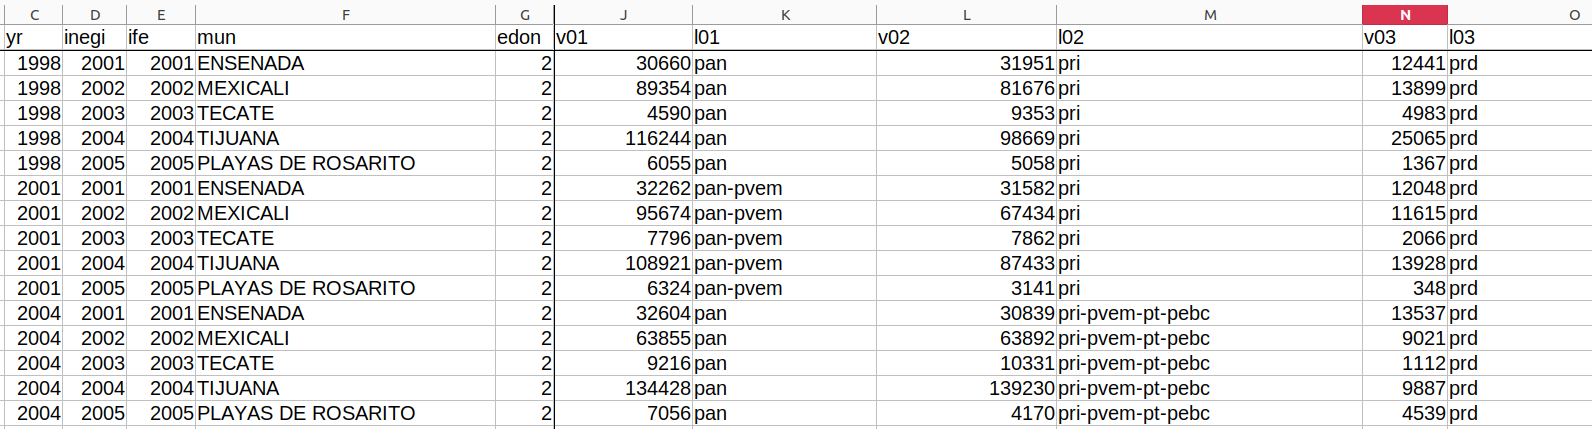
\includegraphics[width=\columnwidth]{pics/eg-spreadsheet-columns.png}
  \caption{Screenshot with a sample of the data organization}\label{F:scrn}
\end{figure}  

Figure \ref{F:scrn} provides a glimpse of the dataset for the five municipalities of Baja California across three electoral cycles: \verb|yr=|1998, 2001, and 2004. Two official municipal identification codes are reported: the census bureau's code (field \verb|inegi|) and the federal electoral authority's code (field \verb|ife|). Researchers wishing to merge census information or vote returns from other elections into the dataset will rely on these codes for matching observations across sources.

Municipal vote returns are stored in column pairs such as \verb|(v01,l01)|, \verb|(v02,l02)|, an so forth, corresponding to the first reported candidate, the second candidate, and so on. Within each pair, the \verb|l| component identifies the party or coalition label, while the \verb|v| component records the total votes won by the party or coalition. For example, in Ensenada's 1998 election, the PRI won a plurality of 31,995 votes ($\texttt{l02} = \texttt{pri}$ indicates that teh PRI's vote total is stored in field $\texttt{v02}$), followed closely by the PAN with 30,660 votes (stored in field $\texttt{v01}$).

This votes--label pair-column structure accommodates four decades of heterogeneity in state'level party systems, compounded by the presence of short-lived electoral coalitions, while using a relatively compact number of spreadsheet columns. The trade-off is that analyzing the performance of a single party across municipalities or along electoral cycles often requires additional data manipulation in order to align that party's vote totals into a common column across observations.\footnote{A standalone R script extracts a simplified matrix, reporting each party's votes in a column that is named after it, for a single state-year's municipal races. The script is located in \verb|code/extract-state-yr-mu-returns.r|.} %\emm{Should write standalone Python script too.}

\section{Pre-election coalitions}\label{S:coalitions}

Electoral coalitions constitute one important obstacle to analysis. Mexican electoral law distinguishes between two forms of pre-electoral alliances that parties may adopt: joint candidacies and formal coalitions. In the former case, voters may cast ballots for any of the parties nominating the joint candidate---or for combinations of those parties---and these votes are subsequently aggregated to determine the candidate's total vote. In formal coalitions, by contrast, voters cast a single vote for the coalition as a whole, and results are reported with without breakdown by member party.

Although these legal distinctions primarily affect the allocation of public party financing, they also substantially complicate voting studies. Researchers must decide whether to treat coalition votes as a pooled total for all member parties or to estimate the contribution of each party separately, which in the case of formal coalitions requires auxiliary assumptions. To facilitate these choices, the repository distributes three separate municipal vote files:

\begin{itemize}
\item \verb|data/aymu1970-on.coalAgg.csv| aggregates votes cast for joint-candidacy coalitions systematically, reporting the candidate's total vote as a single quantity;
\item \verb|data/aymu1970-on.coalSplit.csv| disaggregates the contribution of each coalition member party to the joint candidate's total vote. This procedure relies on the relative vote shares received by each party where the ballot structure provides such information; on coalition agreements between the parties where available and where ballot design does not permit direct disaggregation; or, when neither alternative is feasible, on the relative vote shares obtained by the coalition partners the last time they competed separately in the municipality; and
\item \verb|data/aymu1970-on.csv| reports the raw vote totals exactly as they appear in the primary source---that is, aggregated vote totals for formal coalitions and party-level breakdowns for joint candidacies.
\end{itemize}

\noindent The three files contain records for the exact same set of observations and report identical vote totals. They differ only in the manner in which coalition votes are recorded. Most users will choose between the \verb|coalAgg| and the \verb|coalSplit| versions. Researchers primarily interested in identifying electionb winners and victory margins will generally prefer \verb|coalAgg|, whereas those studying changes in party support over time will likely opt for \verb|coalSplit|.

% THIS FN WAS REMOVED FROM THE FIRST SENTENCE IN THE PARAG ABOVE:
%\footnote{Or near same total votes: whenever the primary source does not offer the coalesced-parties vote breakdown, one artifical vote is added to the raw file, itself split among these parties to keep track of relative contributions.} 

\begin{table}
\resizebox{\textwidth}{!}{
  \begin{tabular}{lrrrrrrrrrrrrc}
    & \mc{12}{c}{Coalition profile relative frequency (\%)} & \\ [-1.8ex]
    \\ \cline{2-12}
    \\ [-1.8ex]
     &      &              &            &            &&   \mc{3}{c}{Double-major}                    &&             &                &       &            \\ \cline{7-9}
     &      & \mc{3}{c}{Major-minor}                 &&               &    \& major-  & \& two       && \mc{2}{c}{Triple-major}      &       & (Mean co- \\\cline{3-5}\cline{10-12}
Cycle&  None&  One         & Two        & Three      &&   Only        &       minor   & maj.-min.    && Only        &  \& maj.-min.  & Total & alitions)  \\ 
     &      &              &            &            &&               &               &              &&             &                &       &            \\ [-1.8ex] \hline
     &      &              &            &            &&               &               &              &&             &                &       &            \\ [-1.8ex] 
 1979--81& 100.0&   ---&    ---&    ---&&    ---&       ---&         ---&&  ---&       ---& 100 & (0.00) \\
 1982--84& 100.0&   ---&    ---&    ---&&    ---&       ---&         ---&&  ---&       ---& 100 & (0.00) \\
 1985--87& 100.0&   ---&    ---&    ---&&    ---&       ---&         ---&&  ---&       ---& 100 & (0.00) \\
 1988--90&  93.9&   6.1&    ---&    ---&&    ---&       ---&         ---&&  ---&       ---& 100 & (0.06) \\ \hdashline
 1991--93&  98.6&   1.3&    ---&    ---&&    ---&       ---&         ---&&  ---&       ---& 100 & (0.01) \\
 1994--96&  99.8&   0.2&    ---&    ---&&    ---&       ---&         ---&&  ---&       ---& 100 & (0.04) \\
 1997--99&  96.4&   2.1&    ---&    ---&&    1.5&       ---&         ---&&  ---&       ---& 100 & (0.04) \\
 2000--02&  77.0&  16.7&    1.8&    ---&&    4.0&       0.4&         ---&&  ---&       ---& 100 & (0.29) \\ \hdashline
 2003--05&  52.8&  29.8&   11.8&    0.4&&    1.8&       3.3&         ---&&  ---&       ---& 100 & (0.65) \\
 2006--08&  20.4&  48.1&   30.2&    0.6&&    0.1&       0.7&         ---&&  ---&       ---& 100 & (1.19) \\
 2009--11&  11.2&  32.3&   14.6&   10.4&&    7.7&      23.8&         ---&&  ---&       ---& 100 & (1.54) \\
 2012--14&   8.6&  50.7&   11.6&    3.6&&    3.5&      22.0&         ---&&  ---&       ---& 100 & (1.39) \\ \hdashline
 2015--17&  24.6&  35.6&   11.0&    0.8&&    6.1&      21.7&         ---&&  0.2&       ---& 100 & (1.16) \\
 2018--20&   6.3&  17.3&   14.7&    7.1&&    6.5&      35.1&        12.9&&  ---&       ---& 100 & (1.86) \\
 2021--23&  26.8&  18.5&    0.2&    ---&&   13.0&       9.5&         0.3&& 18.2&      13.6& 100 & (1.05) \\
 2024--26&  17.4&  19.6&    1.6&    ---&&    6.1&      12.8&         0.7&& 17.1&      24.8& 100 & (1.30) \\ 
         &      &      &       &       &&       &          &            &&     &          &       &        \\ [-1.8ex] 
  \hline
\end{tabular}
}
\caption{Coalitional profile of municipal races by federal election cycle. Cells report the percentage of municipalities in the cycle, and the cycle's mean number of coalitions per race in parentheses. Quantities consider coalitions where one partner at least was a major party (PAN, PRI, PRD, or Morena), ignoring coalitions among minor parties only, which were also quite frequent.}\label{T:coal}
\end{table}

Although coalitions were prohibited at the local level until the mid-1980s and only rarely authorized before the mid-1990s, and rarely authorized up to the mid-1990s, they subsequently became a defining feature of Mexican elections, as shown in Table \ref{T:coal}. Each row of the table reports the coalition profiles observed across municipal elections within a given triennium. With few exceptions resulting from changes in state electoral calendars,\footnote{Subnational electoral calendars varied substantially up to 2015, but have since become increasingly aligned with the federal cycle (see section \ref{S:cal}). Change is discernible in how municipal vote shares align vertically in the right of Figure \ref{F:vpcts}, increasingly clustered over darker and distincter columns that concur with federal elections.} triennial aggregates correspond to one regular election per municipality. A coalition profile is coded as `None' when no coalition competed in the race; as `major-minor' when one, two, or three major parties (PAN, PRI, PRD, or Morena) jointly nominated a municipal ticket with one or more minor parties; as `Double major' when two major parties ran jointly (PAN+PRD, PAN+PRI, or PRI+PRD---Morena never did); and so forth.

Three distinct periods stand out. First, during triennia between 2000 and 2008, at least one major party---and increasingly two major parties---frequently allied minor parties in an effort to gain an advantage in municipal contests. By the end of this period, four out of five municipal elections involved at least one major-minor arrangement. Second, `Double-major' alliances became common between 2009 and 2014, particularly as the PAN and PRD formed anti-PRI coalitions in more than one-fifth of municipalities. During thois period, races without coalitions became increasingly rare. Third, Morena's entry into the party system, especially after 2018, prompted repeated realignments among erstwhile rivals---the PAN, PRI, and PRD---which increasingly formed `triple-major' coalitions to oppose the new dominant force. These broader alliances shrank the number of separate coalitions per municipality by expanding the scope of each coalition, as reflected in the rightmost column of the table, which reports the average number of coalitions per municipality in each triennium (shown in parentheses).

% And the right-most column reports triennial average coalitions per municipality, parenthesized. The mean number of coalitions only surpassed one by 2006--08, up from 0.29 six years before, and rose to a maximum 1.85 in 2018--20. It has declined since.

\begin{figure}
  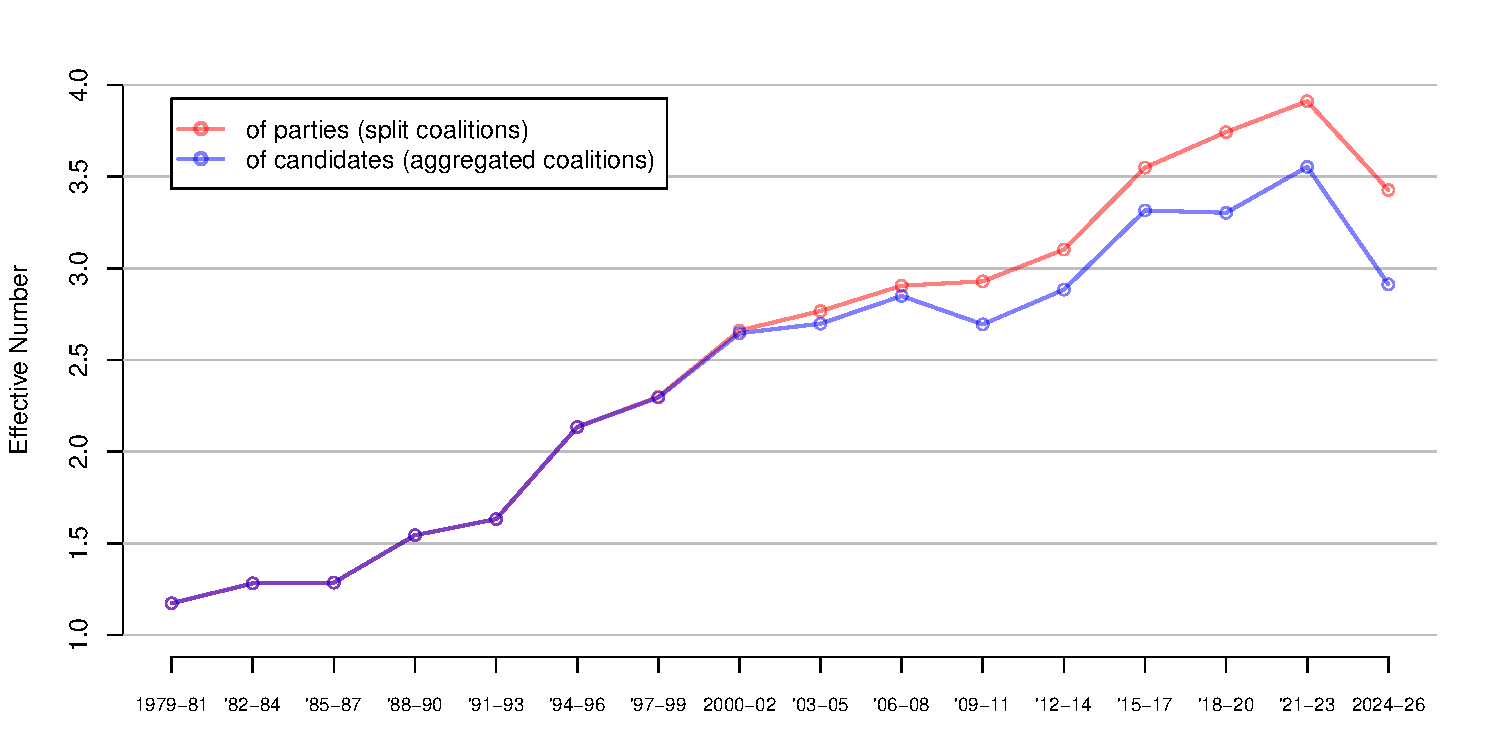
\includegraphics[width=\columnwidth]{../../plots/enp1979-2025.pdf}
  \caption{Municipal party system fragmentation by federal election cycle. Circles report the mean effective number of parties across municipal elections in the cycle.}\label{F:enp}
\end{figure}

% \begin{table}
%   \centering
%   \begin{tabular}{lcc}
%           & \mc{2}{c}{Mean effective number of}     \\ [-1.8ex] 
%     \\ \cline{2-3}
%     \\ [-1.8ex] 
%           & candidates & parties \\
%     Cycle & (aggregated coalitions) & (split coalitions) \\
%     \\ [-1.8ex] \hline 
%     \\ [-1.8ex] 
%  1979--81 &    1.17    &    1.17 \\
%  1982--84 &    1.28    &    1.28 \\
%  1985--87 &    1.29    &    1.29 \\
%  1988--90 &    1.54    &    1.54 \\ \hdashline
%  1991--93 &    1.63    &    1.63 \\
%  1994--96 &    2.13    &    2.13 \\
%  1997--99 &    2.30    &    2.30 \\
%  2000--02 &    2.65    &    2.66 \\ \hdashline
%  2003--05 &    2.70    &    2.77 \\
%  2006--08 &    2.85    &    2.91 \\
%  2009--11 &    2.69    &    2.93 \\
%  2012--14 &    2.88    &    3.10 \\ \hdashline
%  2015--17 &    3.32    &    3.55 \\
%  2018--20 &    3.30    &    3.74 \\
%  2021--22 &    3.55    &    3.91 \\
%  2024     &    2.92    &    3.47 \\
%     \\ [-1.8ex] \hline
%   \end{tabular}
%   \caption{Municipal party system fragmentation by federal election cycle}\label{T:enp}
% \end{table}

Computing the effective number of parties and candidates using the \citet{laakso.taagepera.1979} index---based on the \verb|coalSplit| and \verb|coalAgg| files, respectively---captures the growing incidence of coalitions particularly well. As shown longitudinally in Figure \ref{F:enp}, a gap between the two measures emerged after major-party coalitions became normalized around 2009 and has continued to widen since then. The three distributed file structures therefore provide users with flexibility in handling coalitions according to the needs of their analyses. The repository also includes vote returns for federal and other state-level elections, for which the issues discussed in this section are likewise relevant. This note, however, focuses exclusively on municipal elections.\footnote{The repository also distributes returns to other federal and subnational races at different levels of aggregation. All files are in the \verb|/data| folder: those whose name starts with \verb|df| report federal deputy tallies, \verb|se| are for senate races, \verb|pr| for presidential elections, \verb|go| for gubernatorial, and \verb|dl| for state assemblies. The repository's \verb|README| file has detail on file naming conventions.}

\section{Descriptive statistics}

This section summarizes party vote shares across municipalities nationwide. It purpose is to demostrate that patterns of municipal party support in the distributed files conform to established interpretations of Mexico's unusual democratic transition \citep[e.g.][]{cornelius.1996} and subsequent national political development \citep[e.g.][]{cornelius.weldonCPT2018}. At the same time, the data also reveal patterns distinctive to municipal politics and illustrate several potential applications of the dataset.

\begin{figure}
  \includegraphics[width=\columnwidth]{../../plots/vpct1979-2025.pdf}
  \caption{The electoral evolution of parties in municipal races 1979--2025. Color-coded circles report a given party's vote percentage in a municipal election (slightly x-jittered for visibility). Curves are the vote share that each party won in the median municipality across time (the trend is smoothed for clarity).}\label{F:vpcts}
\end{figure}  

Figure \ref{F:vpcts} provides a group portrait by plotting every municipal elections since 1979 for which data are available, using the split-coalition file. Each small, color-coded circle quantifies a party's vote share in a single municipal election---137,813 observations in total, covering 30,633 non-missing municipal races. At the beginning of the series, the hegemonic party system of the 1960s and 1970s remained largely intact, the PRI's red circles frequently concentrated at 100 percent of the vote, reflecting uncontested dominance \citep{segovia.els1979}. During the 1980s the center-right PAN (shown in blue), along with the emerging left party (shown in gold),\footnote{Several leftist incarnations are coded as PRD in the data: the communists (PCM), PSUM, PMT, and PMS. The PRD was created in only 1989, so this is a simplification of an overcrowded field. But PSUM used PCM's registration, then PMS used PSUM's, and PRD used PMS's. So, technically, these are one and the same party outfit. See \citet{molinar.1991a}.} achieved more than symbolic levels of support only in a very limited number of predominantly urban municipalities.

Opposition parties began gaining momentum after the economic crash of 1982, gradually chanelling social discontent into the electoral arena \citep{molinar.1991a, klesner.Alignment.1993, hiskey.canache.2005, gomezTagle.Estadisticas1990, segovia.dientes-sierra1983}. The trend lines, which smooth party vote shares in the median municipality over time, clearly capture the steady erosion of PRI support and the rise of a dual opposition. Both processes, however, unfolded more slowly in municipal elections than national political developments during the second half of the 1980s might suggest. This apparent anomaly is largely explained by the enormous disparities in municipal population size. Ecological analyses of voting behavior consistently found that the strongest predictor of opposition voting was the unit's proportion of people living in urban areas \citep{ames.1970, lehr.1985, magar.1994, walton.sween-1973, pacheco.VotoUrb.1997}. Although relatively few in number, urban municipalities accounted for a substantial share of the total population. In a rapidly urbanizing society, this relationship foreshadowed the PRI's growing vulnerability. At the same time, it highlighted a major obstacle for emerging parties, as the PRI remained a formidable competitor in smaller, rural, low-turnout municipal enclaves. Until very late in the series, only the PRI possessed the organizational capacity to mobilize voters in these localities. The median municipality remained firmly embedded within such rural enclaves until the mid-1990s.

\begin{figure}
  \centering
  \textbf{A -- Percent municipalities won} \\
  
\includegraphics[width=.9\columnwidth]{../../plots/pctwin1979-2025-legend.pdf} \\
  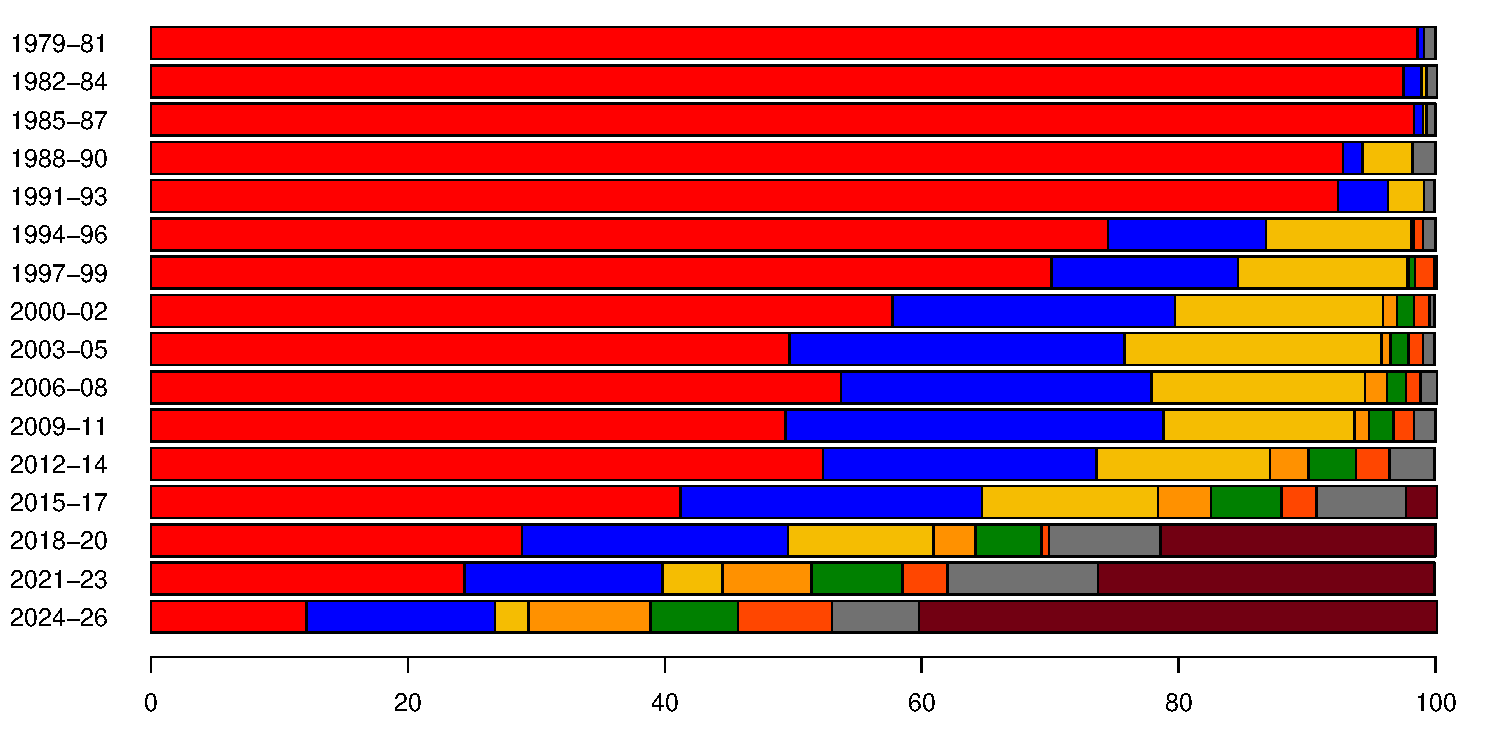
\includegraphics[width=.9\columnwidth]{../../plots/pctwin1979-2025.pdf} \\
  \textbf{B -- Size-weighted percent municipalities won} \\
  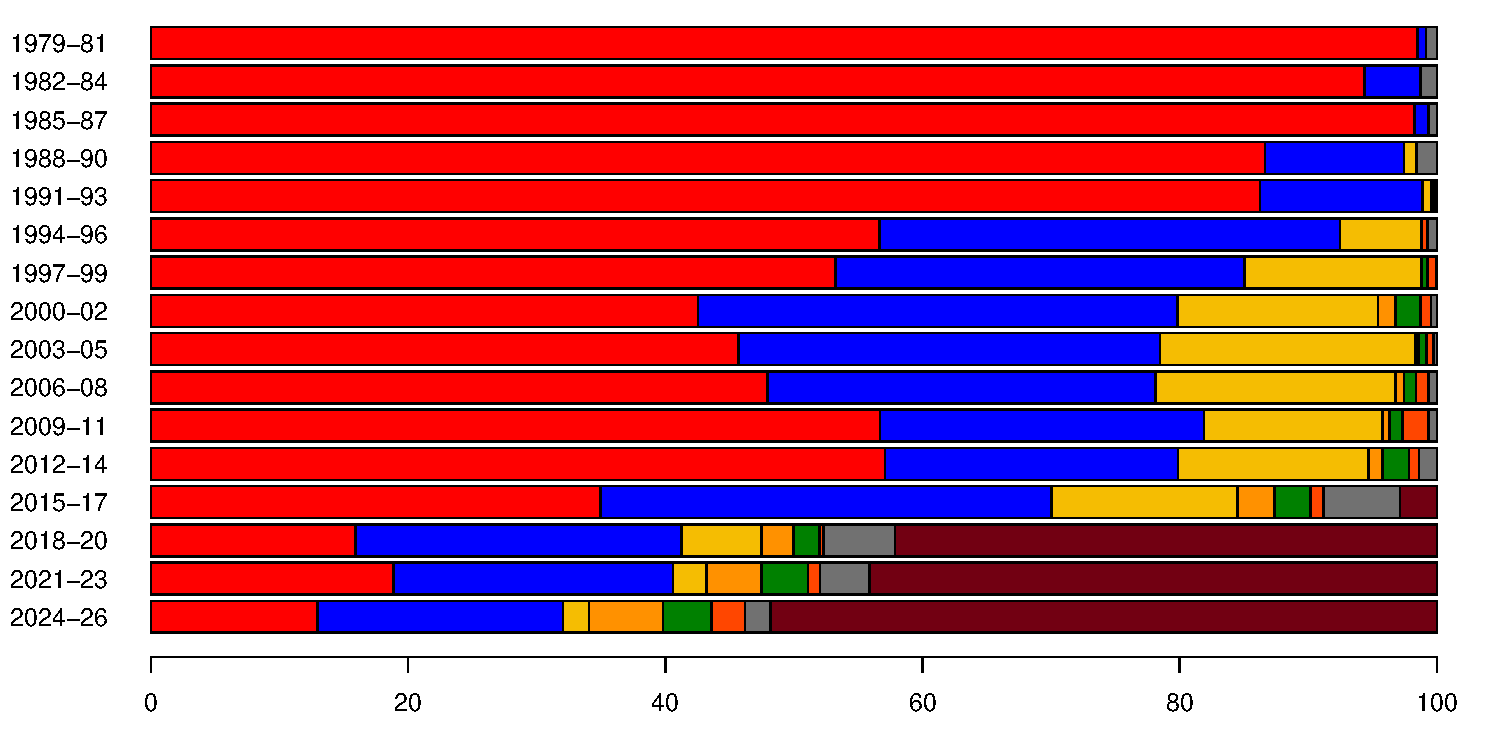
\includegraphics[width=.9\columnwidth]{../../plots/pctwin-popw1979-2025.pdf}
  \caption{Winners by triennial federal electoral cycle. Relative frequencies in panel B are weighted by the municipality's population. See text on how coalition coalition victories were handled.}\label{F:win}
\end{figure}  

Figure \ref{F:win} approaches this lag from a somewhat different angle by focusing on winners in municipal races. In Panel A, each horizontal bar  reports the proportion of municipalities won by each party during a triennial electoral cycle, using the coalition aggregates file. For visual simplicity, victories by coalition tickets are assigned to the major party involved; when two or three major parties competed jointly, the victory is assigned arbitrarily to the largest of them within the corresponding state-cycle. The PRI won nearly all municipal elections in the first three triennia cevered by the series. Its subsequent decline remained barely noticeable as late as 1993, after which electoral losses accelerated but were interrupted by periods of apparent stability: roughly nine out of ten municipal victories between 1988 and 1993, three out of four between 1994 and 1999, and approximately half between 2000 and 2014. The party's final collapse came with Morena's rise to dominance. In the final electoral cycle reported, the PRI won one in ten municipalities only.

Panel B weights municipalities by their share of all registered voters, thereby reflecting the proportion of the national electorate governed by each party in a given cycle. Up to 2008, the PAN's bars are notably larger in panel B than in A, illustrating the party's distinctive urban bias. 

The simultaneous rise of a dual opposition in Figure \ref{F:vpcts} created a coordination problem for anti-PRI voters which helped prolong the PRI's rule even after the erosion of its hegemonic status \citep{magaloni.2006, garrido-phd.2014}.\footnote{The PAN and left's parallel paths are suggestive of what \citet{cox.1997} terms `non-Duvergerian' equilibria: a near tie between challengers that often left the PRI invulnerable in office despite erosion of its support.} Figure \ref{F:triplot} reports the distribution of the three-party vote among the major parties---that is, after subtracting votes cast for candidates outside the PAN-PRI-PRD trio's. Municipalities won uncontested by the PRI cluster around the upper vertex of the triangle, while movements away from that point measure gradual declines in PRI support in favor of the PAN and/or the PRD. The ternary plot reproduces a pattern previously identified in federal elections \citep{marquez.vsData.2014}: between 1989 (the PRD's debutant year) and 2014 (the year before Morena's entry), most observations lie on or very near the edges of the triangle. Although some municipalities lie within the interior, they are comparatively uncommonn. This pattern indicates predominantly local local two-party competition. In other words, opposition support was regionally concentrated: the PRI typically faced a serious challenge from either the PAN or the PRD, but rarely from both simultaneously. The PRI's persistence in municipal elections therefore reflected not merely opposition coordination failures, but also genuine organizational and electoral strength.

\begin{figure}
  \centering
  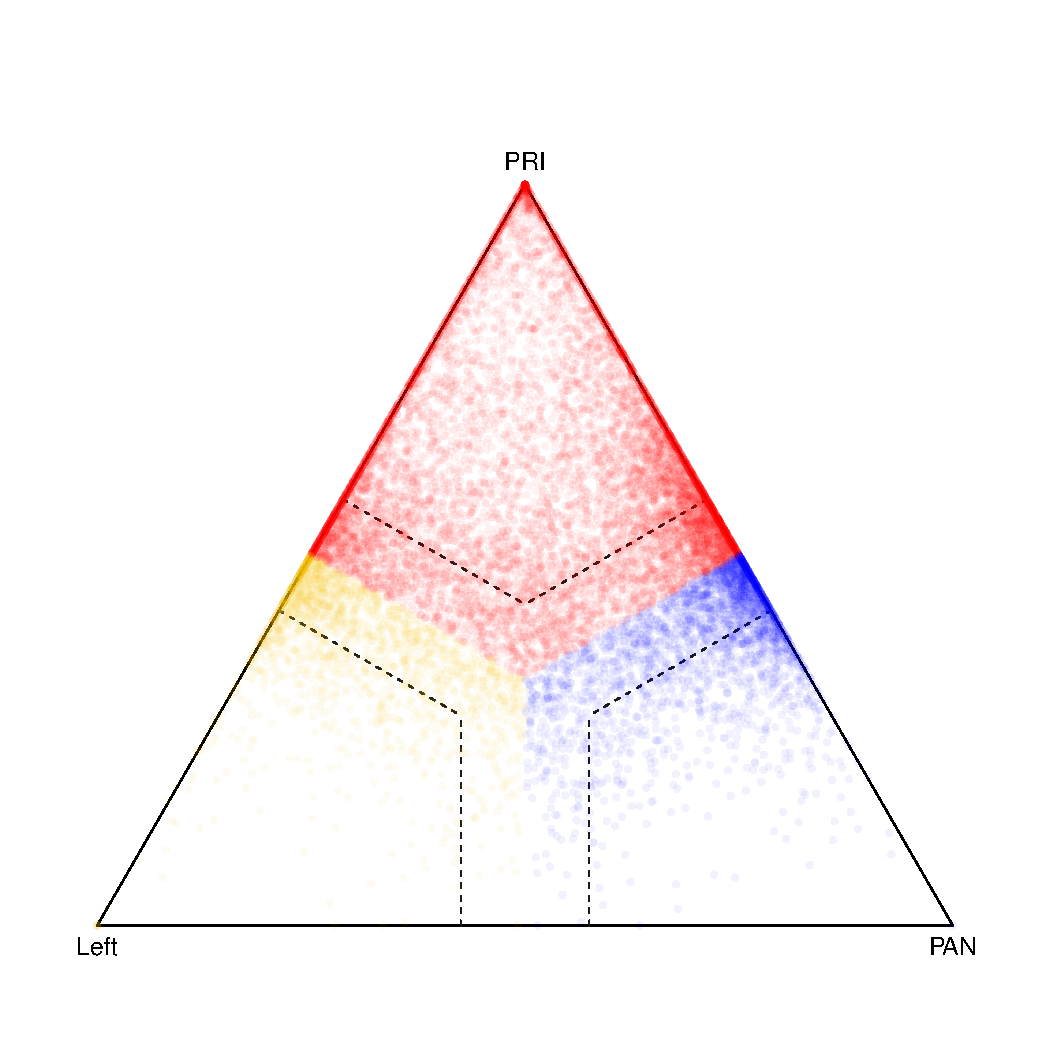
\includegraphics[width=.6\columnwidth]{../../plots/triplot1989-2014-v-mu.pdf}
  \caption{Pre-Morena's predominantly bipartisan rivalries. The ternary plot reports the share of the three-party vote that major parties won in municipal elections in the 1989--2014 period (excluding the Federal District). Points inside the dotted area are marginal municipalities, where the difference between the top-two parties was 10 percentage points or less.}\label{F:triplot}
\end{figure}

The final stage depicted in the data corresponds to the collapse of the party system that structured Mexico's democratic transition \citep{moreno.decisElec.2009}, and the rise of AMLO's Morena. AMLO overcame the chronic factionalism of the Mexican left \citep{bruhn.1997} by launching his new party structured around his personal leadership. The strategy proved successful. Left-wing elite discoordination allowed rival parties to secure unexpected victories in Morena's inaugural 2015 elections. Three years later, however, AMLO's third presidential campaign became a focal point that attracted not just left-wing voters, but independents and defectors from both the PRI and the PAN. Morena's landslide victory in 2018, which gave the party unified control of the federal government and most state governments, prompted the former major parties to form  broad triple-major coalitions in subsequent elections. These desperate efforts achieved little success. Although Morena's rise appears with some lag in Figure \ref{F:vpcts}---because the party first consolidated support in the largest municipalities before expanding into smaller ones---its electoral strength ultimately succeeded in realigning local elites away from the PRI. By the 2024 electoral cycle, the PRI's population-weighted bar in Figure \ref{F:win} had finally fallen below its already diminished share of municipal victories.

\section{Elected officers and reelection}\label{S:incumbents}

Another component of the dataset, distributed in the file \verb|data/aymu1989-on.incumbents.csv|, focuses on elected officeholders. Coverage begins only in 1989, as earlier information is extensively missing. Table \ref{tab:fem} show that municipal government remained an overwhelming male domain until 2015. Nevertheless, the proportion of female municipal executives increased steadily throughout the period before leveling off towards the end of the series.

In 2015, a parity law entered into force, constitutionally rewquiring parties nationwide to nominate equal numbers of female and male candidates across elected offices \citep{piscopo.2016}. The reform more than doubled the number of women elected to municipal office. Even so, women remain underrepresented relative to parity, as femal candidates continue to lose to male candidates more frequently than the reverse. Whether these unequal success rates reflect the difficulty of rapidly recruiting experienced female candidates, the tendency of parties to nominate women in less competitive races, anti-female bias among voters, or other factors remains an important subject for future research. 

\begin{table}
  \centering
  \begin{tabular}{lrl}
    Cycle     & \% women \\ \hline
              &     &  \\ [-1.8ex]
    1988--90$^\dagger$  &   2 &  \\ 
    1991--93  &   4 &  \\
    1994--96  &   4 &  \\
    1997--99  &   4 &  \\
    2000--02  &   5 &  \\
    2003--05  &   5 &  \\
    2006--08  &   6 &  \\
    2009--11  &   8 &  \\
    2012--14  &  11 &  \\
              &     &  \\ [-2.2ex]  \hdashline 
              &     &  \\ [-2.2ex]
    2015--17  &  21 &  \footnotesize{\emph{~~~Gender parity slates adopted}} \\ 
    2018--20  &  28 &  \\
    2021--23  &  27 &  \\
    2024--26  &  28 &  \\
              &     &  \\ [-1.8ex]  \hline 
  \end{tabular} 
  \caption{Municipal glass ceilings dented: female elected municipal presidents. The dashed line separates cycles before and after the nomination of 50 percent women became compulsory for all parties. $\dagger$ Year 1988 from the first election cycle is missing.}\label{tab:fem}
\end{table}

\begin{figure}
  \includegraphics[width=.9\columnwidth]{../../plots/reel-munic2018-23.pdf}
  \caption{Governing party reelection since 2018 by status of the incumbent municipal president. The 2024--26 cycle is dropped because reelection rates remain indetermined. Earlier cycles dropped because they antecede the adoption of municipal consecutive reelection.}\label{F:reel}
\end{figure}  

The incumbents dataset also makes it possible to study patterns of consecutive reelection following its adoption \citep{motolinia-reel-pork2021, lucardi.rosas.Incumbency.2016, lopez.videla.phd.ch1.2021}. Figure \ref{F:reel} presents party reelection rates during the 2018--2023 period conditional on the status of the outgoing municipal president: incumbents who sought reelection are shown in shades of green, incumbents barred by term limits in shades of red, and open-seat races in shades of blue. Several noteworthy patterns emerge:

\begin{itemize}
\item The consistency of the darker green bars, representing incumbents who successfully won reelection, is striking: approximately 21 percent overall, with a variation of only $\pm$ 3 percentage points across parties other than the PRD---which was on its way out after the reform. At first glance, a one-in-five reelection rate may not appear particularly high. However, the combined total of both green-shaded bars captures officeholders displaying static ambition regardless of electoral success: roughly 38 percent overall, with greater variation.
\item The red-shaded bars represent executive officeholders who had already secured reelection in the 2018 cycle and were therefore ineligible to seek a third consecutive term. Because these officials had already demonstrated static ambition, they should be grouped conceptually with the green categories when evaluating the attractiveness of municipal reelection. By the second post-reform electoral cycle, approximately three out of five mayors had attempted to remain in office. This provides a more meaningful indicator of reelection incentives. Particularly striking is the 58 percent rate among Morena incumbents, given that the party's national leadership later supported abolishing the reelection reform beginning in 2030. 
\item The blue-shaded category reports incumbents who retired from office, leaving an average 38 percent of races as open seats. Unfortunately, the dataset does not distinguish whether these withdrawals reflected voluntary retirement or the denial of renomination by the incumbent's party. This limitation represents an important opportunity for future extensions of the dataset.
\end{itemize}
  
\section{The electoral calendar}\label{S:cal}

The final component of the dataset, distributed in the file \verb|data/aymu1989-on.concurrence.csv| relates the timing of each municipal election to the broader electoral calendar. Four dummy variables indicate whether a given municipal election concurred with a gubernatorial, state assembly, presidential, or congressional election.\footnote{See \citet{magarInstReel.2017} and \url{https://github.com/emagar/calendarioReeleccion} for more detail on election calendars in the period. The distrubuted dummies are derived from this parallel repository.} The dataset therefore makes it possible to study coattail effects and other electoral spillovers across races \citep[e.g.,][]{magar.gubCoatMx.2012, ames.1994}. It also enables systematic analysis of changes in state electoral timing, an institutional feature that merits closer scrutiny. Figure \ref{F:cal} shows how the diverse state calendars have gradually become more aligned with the federal calendar over time.

\begin{figure}
  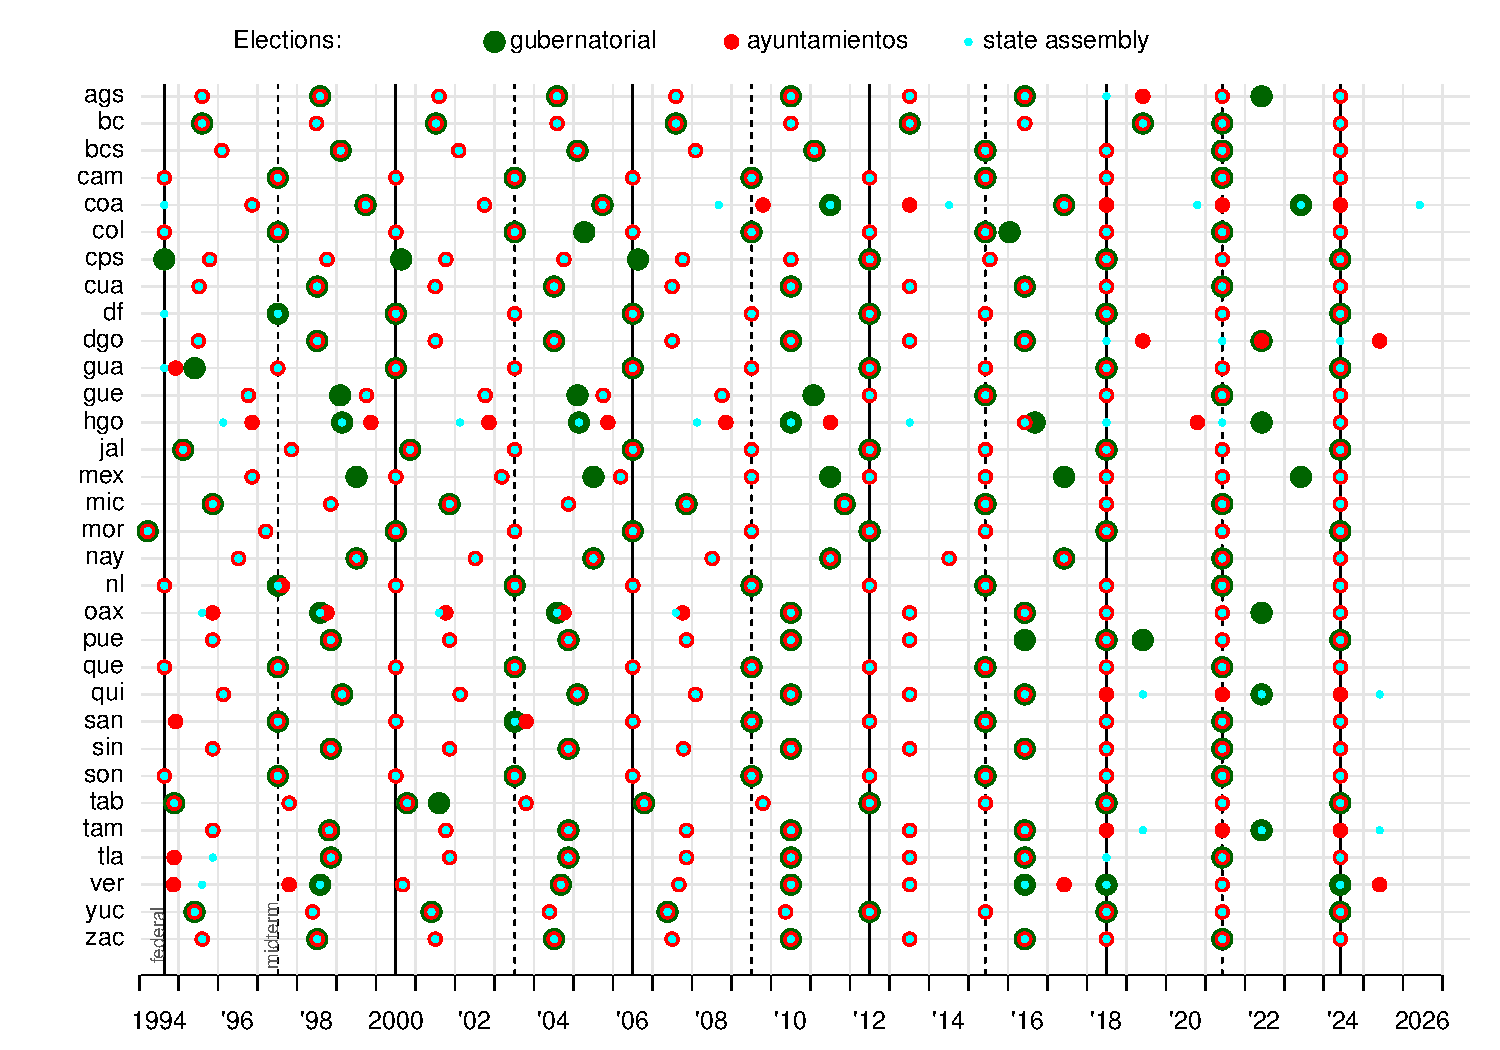
\includegraphics[width=\columnwidth]{../../plots/cal-eng.pdf}
  \caption{Gradual alignment of state and federal electoral calendars 1994--2026. The X-axis measures the timeline, ticks corresponding to January 1 of each year. Vertical black lines indicate the dates of federal races, solid lines for general elections, doted lines for midterm elections. Circumpherences indicate when state elections took place, colored as described in the top legend.}\label{F:cal}
\end{figure}  

%% \section{The measurement of electoral history}
%% Also discusses another dataset in the repository, vhats.

%% \section{Non-fused tickets in Nayarit}
%% Also discusses another dataset in the repository, nayreg.

\section{Conclusion}

The publicly distributed datasets cover roughly half a century of recent Mexican municipal electoral history. The repository includes vote returns for 35,528 non-missing municipal elections across the states beginning with the 1979--81 electoral cycle. The units of observation in the time-series cross-sectional data are municipality--election years, providing a basis for describing and analyzing patterns of substate partisan support. The data also include information of the electoral calendar for 25,456 municipal elections relative to other possibly concurrent contests since the 1990s, as well as the names of 24,088 elected municipal presidents during the same period.

The breadth of systematized information contained in these datasets offers extensive opportunities for empirical analysis. This research note has illustrated how the observed patterns correspond to several well-established findings in the literature on Mexican elections, while also pointing toward numerous promising avenues for future research.

%% Table [[fig:1]] presents two pairs of diagrams for the 2015 (below) and 2018 (above) congressional elections. Each dot represents one municipality, colored according to the winning party, with coordinates in the ternary plot according to the relative votes of the PAN, the PRI, and the left in the federal deputy race (other smaller parties are excluded).\footnote{I must note that, for the left's electoral history (which I arbitrarily call ``Morena'' in the plots and distributed data), I systematically added up the votes of the PRD, PT, and MC up to 2015. I also added Morena's and PES's votes that year. In 2018 the left consisted of Morena, PT, and PES jointly.} 

%% % \begin{figure}
%% % \centering
%% % \caption{Historic expectations and municipal-level vote in two congressional elections}\label{fig:1}
%% % \begin{tabular}{cc}
%% %   
\includegraphics[width=.75\columnwidth]{../assets/img/triplot2018-vhat-mu.png} &
%% %   
\includegraphics[width=.75\columnwidth]{../assets/img/triplot2018-v-mu.png}    \\
%% %   
\includegraphics[width=.75\columnwidth]{../assets/img/triplot2015-vhat-mu.png} &
%% %   
\includegraphics[width=.75\columnwidth]{file:../assets/img/triplot2015-v-mu.png} \\
%% % \end{tabular}
%% % \end{figure}

%% The left side shows the /vote forecasts/. The idea behind this statistic is summarizing the evolution of relative votes in the municipality in five previous elections (2003--2015 in the case of 2018) and using the tendency to project a vote forecast for the current year. Plots in the right side show the actual results observed in both elections.

%% Three features are noteworthy in 2018. The first is the discrepancy between the left and right plots. Either the model does a poor job forecasting, or 2018 was an extraordinary election. History gave license to expect a comfortable PRI victory, both in the number of municipalities won and in margins of victory. Municipalities outside the dotted bands are won by margins of 15 points or more, and the bulk of secure municipalities are red in the forecast, with Morena in a distant second place. In fact, although a significant number of municipalities migrated towards the PAN, it was Morena who showed a clear advantage. PRI was the underachiever. In contrast, the lower left and right plots reveal fewer differences between them---2015 was a more normal election, the past offering much better grounds to forecast. 

%% Second, observed municipalities fled the edges and triangle vertices in 2018. Observations in vertices show a party that has no significant challenger. While those on the edges were bipartisan, whether more (inside dotted bands) or less (outside the bands) symmetric. It is also plain in forecasts that only the PAN--Morena edge was expected to be unpopulated. In practice, however, third party vote rarely collapsed to zero, there was much more dis-coordination than in the past. In fact, the intersection of dotted bands appeared denser and more homogeneous in the right than the left diagram. 

%% Third, the PAN /vs/ left competition was legal tender in 2018. The pattern in competitive municipalities in the last two decades, still visible in the 2015 plots, involved either PRI--PAN or PRI--left rivalries, and rarely PAN--izquierda. It was this pattern that eased electoral alliances between PAN and PRD in sub national races since 2010 that culminated in the Frente they formed in 2018 to nominate a joint presidential candidate. 

%% % # #+CAPTION: Una elección más característica de la partidocracia
%% % # #+NAME:   fig:2
%% % # | file:../assets/img/triplot2015-vhat-mu.png | [[file:../assets/img/triplot2015-v-mu.png]] |


%% % # #+CAPTION: Grano más fino: las secciones
%% % # #+NAME:   fig:3
%% % # | file:../assets/img/triplot2015-v-se.png | [[file:../assets/img/triplot2018-v-se.png]] |

%% Plots in Table [[fig:4]] report /secciones electorales/ and therefore offer much finer-grained than the previous portraits. They introduce the other quantity of interest in this note: parties' /core support/. The idea behind this statistic is measuring the size of the group that has historically supported the party consistently, in good but also in bad years. 

%% % #+CAPTION: Support core and party performance in 2018
%% % #+NAME:   fig:4
%% % | file:../assets/img/resid-pan-2018-vs-pan-core-se.png | [[file:../assets/img/resid-morena-2018-vs-morena-core-se.png]] | file:../assets/img/resid-pri-2018-vs-pri-core-se.png |

%% The horizontal axis in each plot measures the size of party core support groups as a proportion of the /sección/'s electorate. The PRI enjoyed a clear edge over the rest of the parties in the period, with sizable cores in /all/ secciones nationwide. The distributions of the PAN and the left, in contrast, appear concentrated towards the zero---they have relatively few secciones with some unconditional support. 

%% The vertical axis reports the three parties' performance in 2018 (the difference between the observed vote and the forecast). Positive values indicate that the party excelled expectations in the /sección/, negative ones that it under-performed it expectation. The PRI's electoral disaster appears all too clearly in the red plot. There were a few secciones with positive performance, but the density concentrates massively below the horizontal zero line, something that Table [[fig:1]] had hinted. What is truly remarkable is that the dismal performance is directly proportional to the size of the PRI core. President Peña and candidate Meade achieved what seemed, if not impossible, extremely improbable: they alienated the PRI's unconditional voters in 2018. The PAN and the left met expectations in secciones where they have enjoyed with groups of support. Both (especially Morena) over-achieved where they lack important cores, taking away PRI voters. 

%% The note elaborates how statistics were prepared (replication code can be found [[https://github.com/emagar/mxDistritos/code/elec-data-for-maps.r][here]]).

%% % # [[file:https://github.com/emagar/elecRetrns/raw/master/graph/nytAmloPlusAnayaPlusMeadeNegPenaWon.svg]]

%% % # #+CAPTION: PAN
%% % # #+NAME:   fig:6
%% % # #+ATTR_HTML: style="float:right;"
%% % # #+ATTR_HTML: :width 50%
%% % # [[file:../assets/img/resid-pan-2018-vs-pan-core-se.png]]

%% * First differences
%% One common approach to study electoral change is through first differences. Denoting $v_t$ the party's vote share in the municipality or the /sección/, in period $t$, the first difference is simply $d_t = v_t - v_{t-1}$. 

%% $d_t$ is an intuitive quantity, showing the sign and magnitude of change from one election to the next. But, precisely because it compares pairs of consecutive elections only, it misses more dynamic processes in the units. One example, well documented by electoral sociology, is the regression to the mean \citep{campbell.1991,segovia.els1979}. Its detection requires observing the unit through at least three consecutive periods to verify contrary signs in $d_{t+1}$ and $d_t$. The study of secular change in the Mexican party system in the last quarter of century calls for deeper historical perspective. 

%% (First differences appear in the fields ~d.pan~, ~d.pri~, and ~d.morena~ in the distributed data.)

%% * The recent linear tendency
%% One way of adopting it is with /vote forecasting/ from tendencies discernible in the previous five congressional races \citep{magar.gubCoatMx.2012}. I summarize the central tendency of the recent historical vote by means of linear estimation in time, fitting a straight line for each year analyzed and each party in the municipality or /sección electoral/. 

%% The slope of the fitted line (the tendency) serves to extrapolate the party's electoral support to the future. For instance, to get the vote share that the recent past predicts for a party in unit $u$ for 2018, I estimate the following equation 

%% \begin{equation}
%% v_{ut} = a_u + b_u \times t + \text{error}_{ut}, \; t = 2003, \ldots, 2015
%% \end{equation}\label{ts-eq}

%% that I then use to predict $\hat{v}_{u2018} = \hat{a}_u + \hat{b}_u \times 2018$. This is an out-of-sample prediction of the party's vote share, it can be compared to the party's actual vote share in 2018 to gauge whether or not the unit approximates the historical record. For the 2015 forecast the sample shifts one period to become $t = 2000, \ldots, 2012$, and so on an so forth for previous years. I distribute forecasts for 2009, 2012, 2015, and 2018, which involved fitting about 10 thousand municipal regressions and more than 250 thousand sección-level.

%% (Vote forecasts appear in the fields ~vhat.pan~, ~vhat.pri~, and ~vhat.morena~ of the distributed data.)

%% * The party's support core
%% The other historical statistic is the parties' core support in the unit. Its definition stems from classifying voters in three categories: (1) support groups, that in the past have consistently supported the party; (2) opposition groups, that have consistently supported another party; and (3) swing groups, that have neither consistently supported nor consistently opposed the party \citep{cox.mccubbins.1986}. The party core consists of the support groups. 

%% I use the procedure by Díaz Cayeros /et al/. (2016) to estimate this core. If $\bar{v}_t$ denotes the party's mean support across all units in period $t$,\footnote{The analyzed unit $u$ should be dropped from period $t$'s mean in order to not include the dependent variable in the right side of equation \ref{ts-eq}. I do not drop it due to the large number of municipal or seccional units (each contributing a fraction to the mean) and the use of vote shares (so large units are watered down): this refinement's impact should be negligible in each mean value.} for each party in each unit I fit

%% \begin{equation}
%% v_{ut} = \alpha_u + \beta_u \times \bar{v}_t + \text{error}_{ut}, \; t = 1994, \ldots, 2018.
%% \end{equation}\label{alpha-eq}

%% $\beta_u$ measures the effect that national party tides have on the party's vote in unit $u$. For instance, $\hat{\beta}_u=1$ estimates that for every percentage point that the party wins or loses nationally in year $t$, it also wins or loses one percentage point in the unit; $\hat{\beta}_u=0$, on the other hand, would indicate the unit's full isolation form national swings. It is therefore a measure of party volatility in the municipality or /sección/ (analogous to \href{https://www.investopedia.com/terms/v/volatility.asp}{"beta volatility"} in the financial literature). 

%% The $\alpha$ coefficient estimates the core size: expected support in unit $u$ in the hypothetical case that the party receives no vote at the national level. For instance, $\hat{\alpha}=.4$ would indicate that, in the starkest of scenarios, 40% of the electorate in the municipality is unconditional to the party---which would indeed be a core of substantial size.

%% A critique that can be anticipated towards this measure of the party's support core is its extreme counter-factual nature \citep{king.zeng.counterfactuals2006pa}. It deserves rigorous scrutiny, something I plan doing in the near future. 

%% (The parties' core support appears in the fields ~alphahat.pan~, ~alphahat.pri~, and ~alphahat.morena~ of the distributed data. Party volatility in ~betahat.pan~, ~betahat.pri~, and ~betahat.morena~.)

%% * Compositional variables
%% I close with an important feature of the model specifications, associated with the \emph{compositional} nature of electoral returns. Compositional variable are quantitative descriptions of the parts of a whole. They therefore have two characteristics: (1) they are proportions that (2) add up to unity.\footnote{Formally, the compositional are random variables subject to two constraints: 
%% $0 \leq v_p \leq 1 \; \forall \; p \in P \; \; and \; \; \sum_P v_p = 1.$.} 

%% When estimating parties separately, the challenge of equations 1 and 2 is to avoid forecasting vote shares less than zero or greater than one; and that the sum of party forecasts equals 1. To achieve this, \citet{aitchison.1986} proposes substituting vote shares by log-ratios in the analysis. Arbitrarily setting the PRI as the reference party, define party $p$'s vote relative to the PRI as 

%% $r_p = \frac{v_p}{v_{\text{pri}}}.$

%% A value $r_p=1$ would indicate a tie between the party and the PRI, while $r_p>1$ that it finished ahead of the PRI in the proportion that the value reveals. 

%% Thus, equation 1 is re-specified as

%% $\ln r_{put} = a + b \times t + \text{error}$

%% y equation 2 as

%% $\ln r_{put} = \alpha + \beta \times \bar{r}_{pt} + \text{error}.$

%% Applying the natural logarithm attenuates the effect of extreme values of the regressor on the dependent variable, similar as a logit regression would. Models fitting was done with ordinary least squares. 

%% Coefficient estimates requires transformation to collect party vote shares. Illustrating with a three-party caste, it is trivial that 

%% \begin{equation}
%% \hat{v}_p = \frac{\hat{r}_p}{1 + \hat{r}_{\text{pan}} + \hat{r}_{\text{morena}}} \; \text{and} \;
%% \hat{v}_{\text{pri}} = \frac{1}{1 + \hat{r}_{\text{pan}} + \hat{r}_{\text{morena}}.}
%% \end{equation}

%% %% \begin{equation}
%% %% \begin{split}
%% %% v_{\text{pri}} + v_{\text{pan}} + v_{\text{morena}} & = 1 \\
%% %% v_{\text{pri}} & = 1 - v_{\text{pan}} - v_{\text{morena}} \\
%% %% 1 & = \frac{1}{v_{\text{pri}}} - \frac{v_{\text{pan}}}{v_{\text{pri}}} - \frac{v_{\text{morena}}}{v_{\text{pri}}} \\
%% %% \end{split}
%% %% \end{equation}

%% These are the quantities that the distributed data report. 


%% % # Fácil de implementar en R:
%% % # a = voto partido unidad 1
%% % # A = voto efec unidad 1
%% % # N = 3 unidades
%% % #
%% % # tengo
%% % # v.bar = 1/3 * (a/A + b/B + c/C)
%% % #
%% % # quiero
%% % # v.bar.sin.aA = 1/2 * (b/B + c/C)
%% % #
%% % # hago
%% % # 1/3 * (a/A + b/B + c/C) =      v.bar
%% % #        a/A + b/B + c/C  =  3 * v.bar
%% % #              b/B + c/C  =  3 * v.bar - a/A
%% % #       1/2 * (b/B + c/C) = (3 * v.bar - a/A) * 1/2 = v.bar.sin.aA
%% % #
%% % # v.bar.sin.aA = (N * v.bar - a/A) * 1/(N-1)

\newpage

\bibliographystyle{apsr}
\bibliography{/home/eric/Dropbox/mydocs/magar}


\end{document}
